\appendix
\section{Prompts}
\label{app:prompts}

\begin{table}
\resizebox{\textwidth}{!}{
\begin{tabular}{p{2cm}|p{4cm}|p{4cm}|p{4cm}}
\toprule
\textbf{Task} & \textbf{Generate Rule ($\phi_{rg}$)} & \textbf{Follow Rule ($\phi_{rf}$)} & \textbf{Direct Few-shot ($\phi$)} \\
\midrule
List Function & Consider the following input-output examples. Both the input and the output are Python lists. Based on the example shown below, identify the rule that can be used to convert the input into the output. Your output should solely contain the rule. & The following problem contains a rule and an input. Use the rule to produce the output from the given input. Your output should solely be a valid Python list that represents the output. No other text or description should be present. & Consider the following input-output examples. Both the input and the output are Python lists. Based on the example shown above, produce the output from the following input. No other text or description should be present. \\ \midrule
1D ARC & Consider the following input-output examples. Both the input and the output are Python lists. Based on the example shown below, identify the rule that can be used to convert the input into the output. Your output should solely contain the rule. & The following problem contains a rule and an input. Use the rule to produce the output from the given input. Your output should solely be a valid Python list that represents the output. No other text or description should be present. & Consider the following input-output examples. Both the input and the output are Python lists. Based on the example shown above, produce the output from the following input. No other text or description should be present. \\ \midrule
ACRE & Generate a rule that maps the following inputs to their corresponding outputs. Each example is an input-output pair. The input is a list of objects. The presence of certain objects will trigger the light to turn on. The output is either 'on', 'off', or 'undetermined', indicating the state of the light or if the state of the light cannot be determined. Your output should solely contain the rule. & Generate an output corresponding to the given input based on the following rule. Each example is an input-output pair. The input is a list of objects. The presence of certain objects will trigger the light to turn on. The output is either 'on', 'off', or 'undetermined', indicating the state of the light or if the state of the light cannot be determined. & Consider the following few-shot examples. Each example is an input-output pair. The input is a list of objects. The presence of certain objects will trigger the light to turn on. The output is either 'on', 'off', or 'undetermined', indicating the state of the light or if the state of the light cannot be determined. Based on the example shown above, produce the output from the following input. No other text or description should be present. \\ \midrule
MiniSCAN & Generate rules that map the following inputs to their corresponding outputs. Specify the priority of the rules if necessary. Try to make your rules as minimal and generally applicable as possible. & Generate an output corresponding to the given input based on the following rules. The output is a sequence of tokens joined by spaces. & Consider the following input-output few-shot examples. Based on the example shown above, produce the output from the following input. No other text or description should be present. \\ 
 \bottomrule
\end{tabular}
}
\caption{In-context learning prompts}
\label{tab:prompts}
\end{table}

\section{Decoding Strategy}
\label{app:temperature}


\begin{figure}[htbp]
    \centering

    \begin{subfigure}[b]{0.49\textwidth}
        \centering
        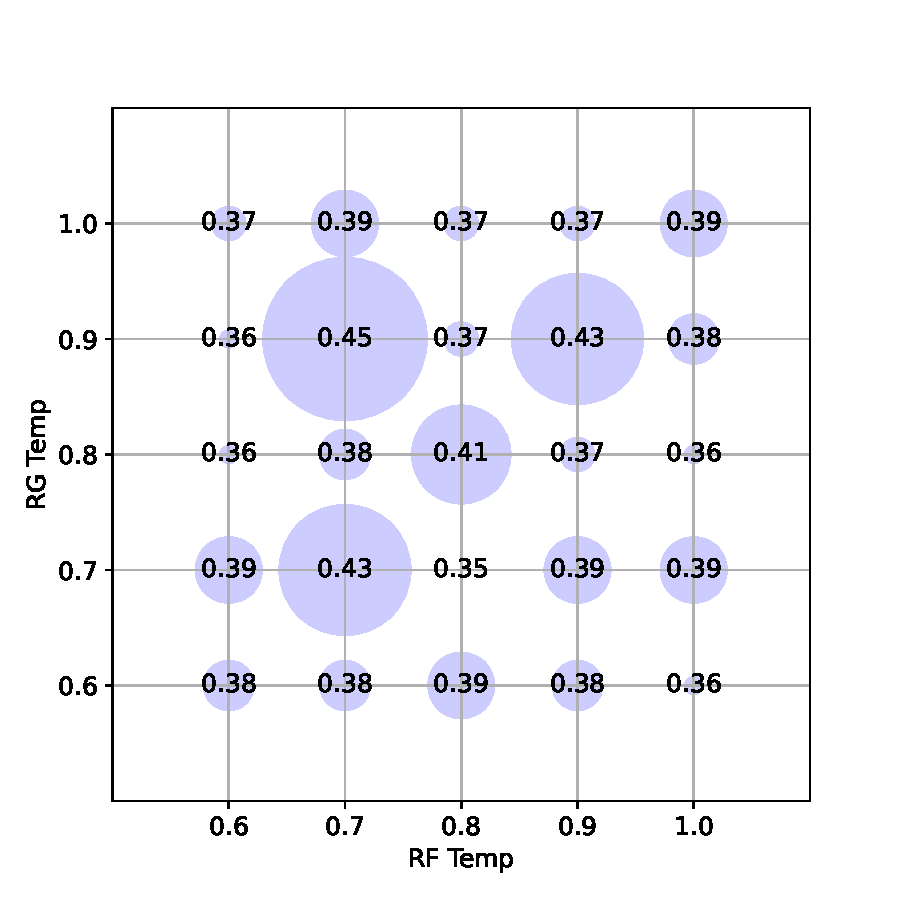
\includegraphics[width=\linewidth]{Figures/temperature_search1.pdf}
        \caption{\proposed-Mistral}
    \end{subfigure}
    \hfill
    \begin{subfigure}[b]{0.49\textwidth}
        \centering
        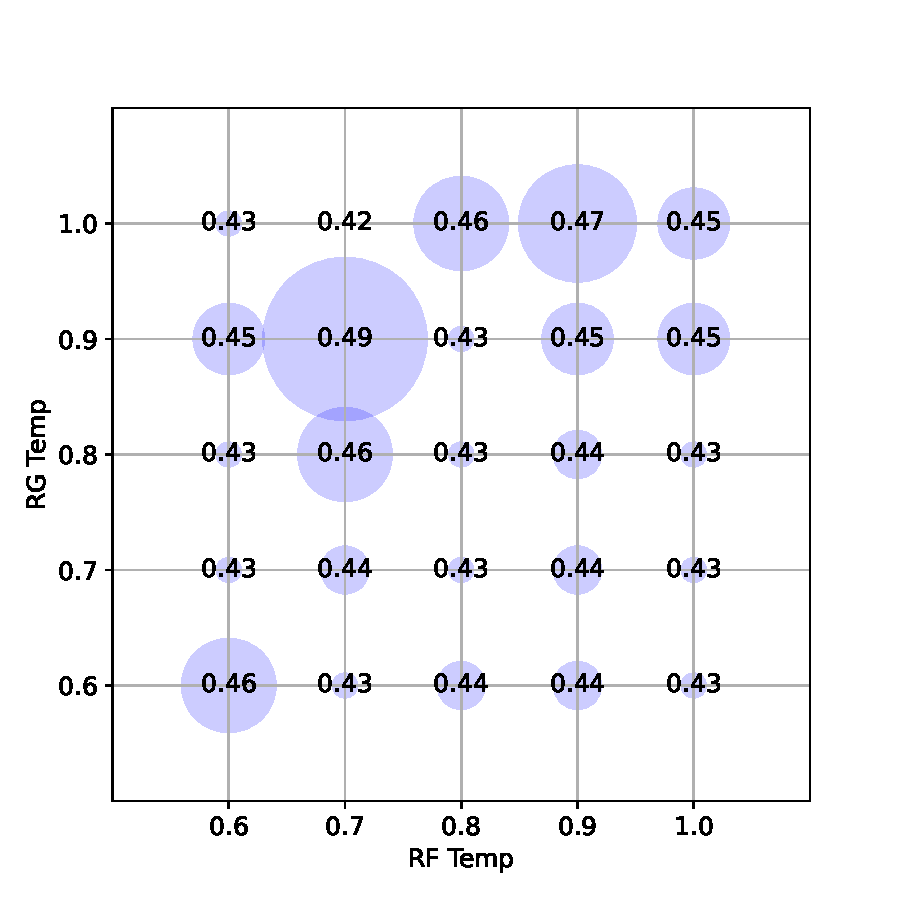
\includegraphics[width=\linewidth]{Figures/temperature_search2.pdf}
        \caption{\proposed-Llama}
    \end{subfigure}

    \caption{The impact of decoding temperature on the performance of a) \proposed-Mistral b) \proposed-Llama on List function task. We perform grid search within the range between $0.6$ and $1.0$ for both rule generation and rule following and find the best performance for a rule generation temperature of $0.9$ and rule following temperature of $0.7$.}
    \label{fig:temperature_search}
\end{figure}

\section{Hypotheses Quality Analysis}
\label{app:data_quality}

\begin{figure}[htbp]
    \centering

    \begin{subfigure}[b]{0.49\textwidth}
        \centering
        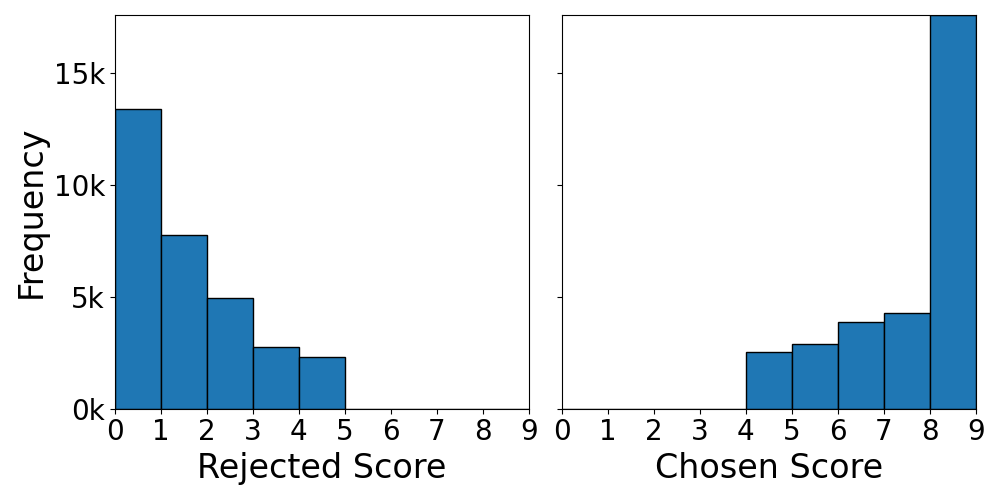
\includegraphics[width=\linewidth]{Figures/List_Function_scores.png}
        \caption{List Function (n=8,d=3)}
    \end{subfigure}
    \hfill
    \begin{subfigure}[b]{0.49\textwidth}
        \centering
        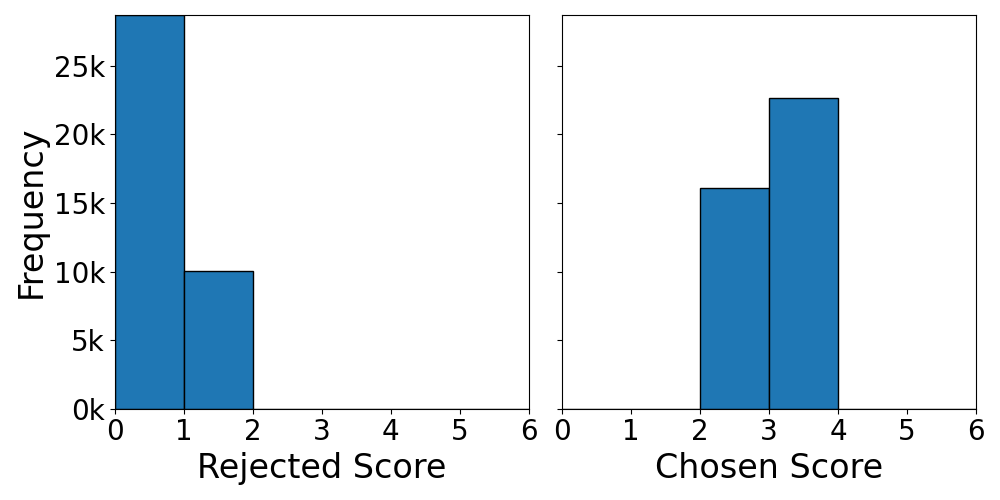
\includegraphics[width=\linewidth]{Figures/1D_ARC_scores.png}
        \caption{1D ARC (n=3,d=1)}
    \end{subfigure}

    \vskip\baselineskip
    \begin{subfigure}[b]{0.49\textwidth}
        \centering
        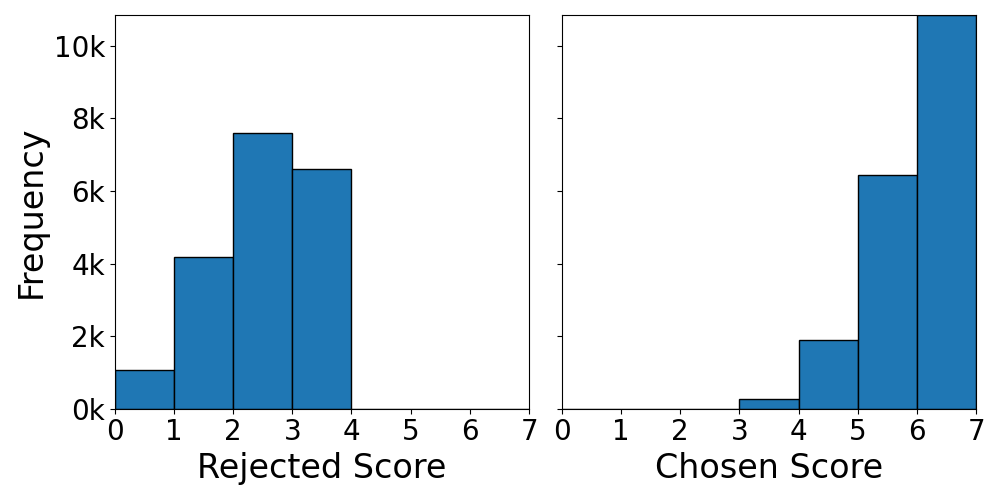
\includegraphics[width=\linewidth]{Figures/ACRE_scores.png}
        \caption{ACRE (n=6,d=2)}
    \end{subfigure}
    \hfill
    \begin{subfigure}[b]{0.49\textwidth}
        \centering
        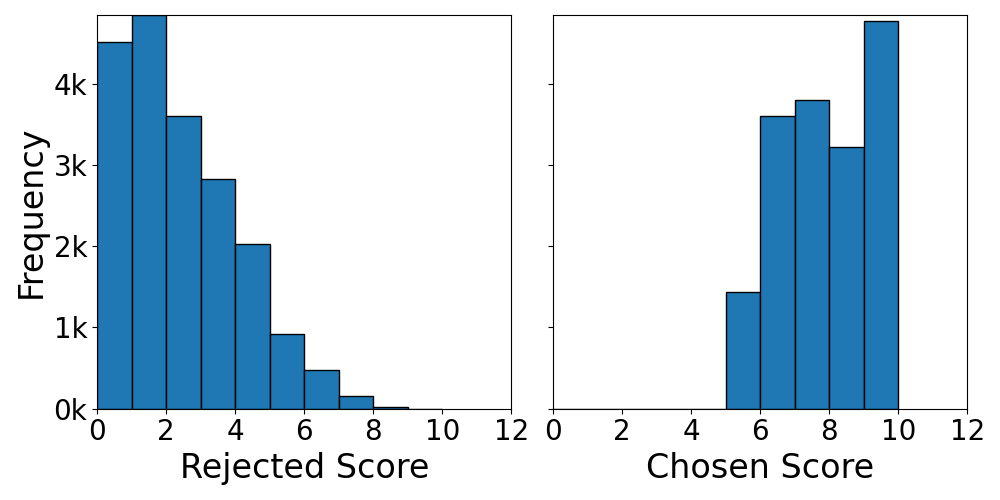
\includegraphics[width=\linewidth]{Figures/MiniSCAN_scores.png}
        \caption{MiniSCAN (n=14,d=4)}
    \end{subfigure}

    \caption{Score distribution of chosen and rejected rules in the augmented dataset via noisy fitness estimation. $n$ denotes the maximum number of few-shot demonstrations, and $d$ denotes the minimum score difference between a (chosen, rejected) rule pair.}
    \label{fig:data_quality}
\end{figure}